\section{Evaluation}

Our experiment with \CoBBl~aims to answer the following questions:
\begin{enumerate}
  \item How does \CoBBl~perform compare to state-of-the-art direct-translators on (a) compiler time, (b) prover time (c) verifier time, and (d) proof size? \label{q:performance-dt}
  \item How does \CoBBl~perform compare to state-of-the-art virtual machines on the same metrics as in question \ref{q:performance-dt}? \label{q:performance-vm}
  \item To what extent do improvements introduced through \CoBBl's block-based abstractions outweight the overheads? \label{q:tradeoff}
  \item How effective are \CoBBl's static optimizations in improving proof runtime and size? \label{q:optimization}
\end{enumerate}

We choose CirC~\cite{ozdemir20circ} as the baseline for state-of-the-art direct translator, and Jolt~\cite{arun23jolt} as the baseline for virtual machine. \red{[XXX: Need justification?]} We conduct the experiments on implementations of \CoBBl, CirC and Jolt across several benchmarks.

\subsection{Implementation}
\red{[XXX: Will there be a separate implementation section? Some details might be interesting to go through]} We base the frontend compiler of \CoBBl~on top of existing infrastructure of CirC, our direct translator baseline, as CirC contains most underlying functionalities required by \CoBBl~(in particular, conversion of high-level languages to constraints). On top of CirC, we implement \CoBBl's frontend through 7000 lines of Rust code: dividing a program in to segments, performing all optimizations on each segment, and repackaging each segment as individual programs recognizable by CirC's direct translator. We apply minimal modification to CirC's internal codebase to ensure fairness of comparison.

The backend proof system for \CoBBl~is a custom variant of Spartan~\cite{setty19spartan}, the same proof system used by our two baselines. We modify Spartan through 7000 lines of Rust code to support parallel execution of all program segments, but leave most internal logic untouched.

\subsection{Baselines and Benchmarks}
\paragraph{CirC} We modify CirC to support branching statements to align with our benchmarks, but using exclusively existing functionalities. Apart from updates to the parser and input format, everything else stays the same as the original codebase~\cite{circ_codebase}.

\paragraph{Jolt} Our Jolt evaluation uses the released codebase~\cite{jolt_codebase}.

\paragraph{\CoBBl~without optimization} To answer question \ref{q:optimization}, we disable all non-essential \CoBBl~optimizations (most importantly, block merge and register spilling) and conduct tests across all benchmarks.

\paragraph{Benchmarks} Figure \ref{fig:benchmark_overview} lists our benchmarks. We implement each benchmark in two programming languages: the Zokrates version is used by \CoBBl~and CirC, while Jolt uses the Rust version, compiled using release mode (\code{--release}). As Zokrates closely resembles Rust, the two versions of each benchmark are identical up to grammatical difference. Since CirC generally performs far worse than Jolt, we choose a different set of parameters when comparing \CoBBl~against CirC and Jolt. All benchmarks except for Poseidon are computed exclusively using 32-bit registers -- the native instruction set for Jolt -- to ensure its maximum efficiency. We explore the special scenario introduced by Poseidon later in the section.

\paragraph{Special Benchmark} To answer question \ref{q:tradeoff}, we conduct a separate test on the Find Min benchmark, recording performance of CirC and \CoBBl~for array length ranging from 200 to 1600.

\begin{table}[t]
  \begin{tabular}{l l l}
    \centering
    \textbf{Benchmarks} & \textbf{Parameters} & \textbf{Type} \\
    \hline \\
    \makecell[l]{Min value in an array \\ (Find Min)} & \makecell[l]{\emph{v. CirC}: len = 1200 \\ \emph{v. Jolt}: len = 1200} & 32-bit \\
    \vspace{2\baselineskip}\\
    \makecell[l]{Matrix Multiplication \\ (Mat Mult)} & \makecell[l]{\emph{v. CirC}: size = 8x8 \\ \emph{v. Jolt}: size = 16x16} & 32-bit \\
    \vspace{2\baselineskip}\\
    \makecell[l]{KMP pattern match \\ (Pat Match)} & \makecell[l]{\emph{v. CirC}: pat / txt = 48 / 480 \\ \emph{v. Jolt}: pat / txt = 48 / 480} & 32-bit \\
    \vspace{2\baselineskip}\\
    \makecell[l]{Largest common subsequence \\ (LCS)} & \makecell[l]{\emph{v. CirC}: len = 5 \\ \emph{v. Jolt}: len = 30} & 32-bit \\
    \vspace{2\baselineskip}\\
    \makecell[l]{RLE encode + decode \\ (RLE)} & \makecell[l]{\emph{v. CirC}: len = 20 \\ \emph{v. Jolt}: len = 60} & 32-bit \\
    \vspace{2\baselineskip}\\
    \makecell[l]{Sha-256 Hashing \\ (Sha256)} & \makecell[l]{\emph{v. CirC}: len = 1 \\ \emph{v. Jolt}: len = 6} & 32-bit \\
    \vspace{2\baselineskip}\\
    \makecell[l]{Poseidon Hashing \\ (Poseidon)} & \makecell[l]{\emph{v. CirC}: len = 3 \\ \emph{v. Jolt}: len = 6} & field \\
  \end{tabular}
  \caption{Overview of benchmarks.}
  \label{fig:benchmark_overview}
\end{table}

\subsection{Setup}
Our testbed is a MacBook pro running on a 10-core M1 Max chip and 64 GB of memory. For each system and benchmark, we execute the computation 5 times, recording compiler, prover, verifier time, and proof size and averaging the results. 

\subsection{Method and Results}
\subsubsection{Comparing Runtime of \CoBBl~with CirC}
We present the performance comparison in figure \ref{fig:performance_dt}. \red{[XXX: Fix overlap on graph]} For each benchmark, we measure the compiler, prover, and verifier time of \CoBBl~as speedups from CirC. Since runtime of \CoBBl~scales with program input but runtime of CirC stays the same, we derive three scenarios regarding to the workload of \CoBBl:
\begin{itemize}
  \item \textbf{CoBBl For} executes the exact same program as CirC, where the size of the array and number of iterations of each loop is statically bounded.
  \item \textbf{CoBBl 75} sets the array size to be 75\% of the statically inferred upper bound. Subsequently, all loops are executed only 75\% of the statically inferred number of iterations. \red{[XXX: Need to talk about the exception of Mat Mult.]}
  \item \textbf{CoBBl 50} is similar to CoBBl 75, but with only 50\% array size.
\end{itemize}

To enhance CirC's performance, we allow polynomial commitment in both \CoBBl~and CirC to run in multicore. We note that since polynomial commitment takes up a higher percentage of CirC's runtime than \CoBBl, such a setup is more beneficial towards CirC.

\begin{figure*}[t]
  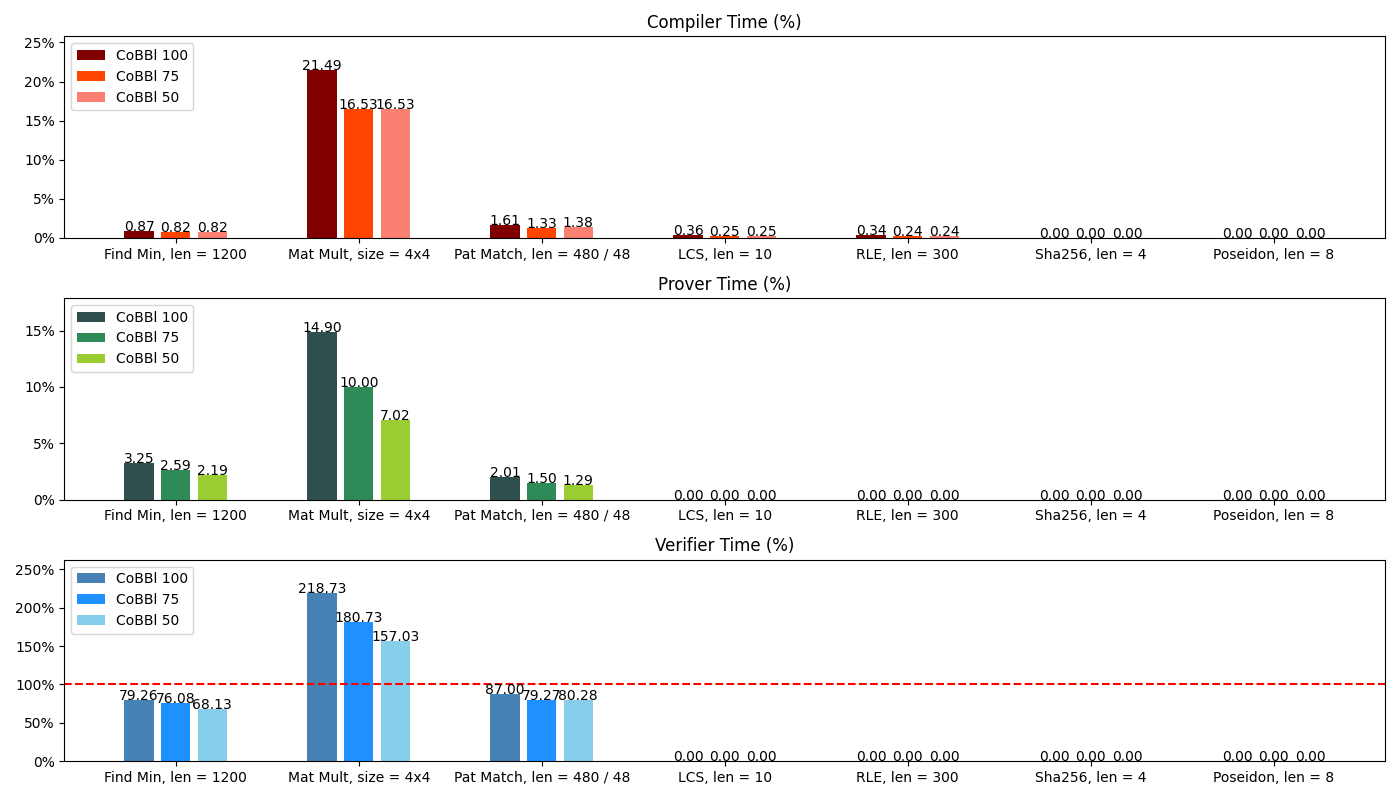
\includegraphics[width=\textwidth]{graph/fig_eval_circ.png}
  \caption{Runtime comparison between \CoBBl~and CirC.}
  \label{fig:performance_dt}
\end{figure*}